\documentclass[12pt, a4paper]{book}
\usepackage[a4paper, total={6in, 8in}]{geometry}
\usepackage[english]{babel}
\usepackage{ragged2e}
\usepackage{ragged2e}
\usepackage{fancyhdr}
\usepackage{lastpage}
\usepackage{listings}
\usepackage{color}
\usepackage{graphicx}
\usepackage{hyperref}
\graphicspath{{images/}}

\def\thesection{\Roman{section}}
\def\thesubsection{\Roman{section}.\Roman{subsection}}
\def\thesubsubsection{\Roman{section}.\Roman{subsection}.\Roman{subsubsection}}

\pagenumbering{arabic}

\pagestyle{fancy}
\fancyhf{}

\lfoot{{\small Rev. 1.0}}
\rfoot{{\small Page \thepage \hspace{1pt} of \pageref{LastPage}}}

\title{\textbf{{\LARGE G.A.I.A.} \\ User Manual \\ {\small v1.0.0} }}
\author{D.A.M.O.F.}
\date{September 2022}

\setcounter{secnumdepth}{0} % sections are level 1

% MACROS
\newcommand*{\thead}[1]{\multicolumn{1}{|c|}{\bfseries #1}}

\begin{document}
\maketitle

\addtocontents{toc}{\protect\setcounter{tocdepth}{-1}}
% From this point on, only show up to \chapters in the ToC
\newpage
\section {Abstract}

\begin{justify}
This user manual describe how to use G.A.I.A. and more in details how to control the behaviour using configuration file.
\end{justify}


\addtocontents{toc}{\protect\setcounter{tocdepth}{3}}
% From this point on, only show up to \subsection in the ToC

% Table of Contents
\tableofcontents

\addtocontents{toc}{\protect\setcounter{tocdepth}{-1}}
% From this point on, only show up to \chapters in the ToC

\newpage
\begin{center}
\textbf{{\large Document Management}}
\end{center}

\begin{table}[h]
\centering
	\begin{tabular}{|l|l|c|}
	\hline
	Author & FDA & 16/09/2022 \\
	\hline	
	Issued by & & \\
	\hline
	Revised by & & \\
	\hline
	Approved by & & \\
	\hline
	\end{tabular}	 	
\end{table}

\begin{center}
\textbf{{\large Document Status Sheet}}
\end{center}

\begin{table}[h]
\centering
	\begin{tabular}{|c|c|l|}
	\hline
	\thead{ Issue } & \thead{ Date } & \thead{ Comment } \\
	\hline	
	1.0 & 23/09/2022 & First Release \\
	\hline
	& & \\
	\hline
	& & \\
	\hline
	\end{tabular}	 	
\end{table}

\begin{center}
\textbf{{\large Document Change Record}}
\end{center}


\begin{table}[h]
\centering
	\begin{tabular}{|l|l|c|c|}
	\hline
	\thead{ Issue } & \thead{ Reason for change } & \thead{ Paragraph } & \thead{ Type of Modification } \\
	\hline	
	& & & \\
	\hline
	& & & \\
	\hline
	& & & \\
	\hline
	\end{tabular}	 	
\end{table}



\addtocontents{toc}{\protect\setcounter{tocdepth}{3}}
% From this point on, only show up to \subsection in the ToC

\newpage
\section{Introduction}

The GTFS is largely used for 

\subsection{Purpose}
\subsection{Scope}

\subsection{Definitions}
\subsection{Abbreviations}
\subsection{Reference Documents}
{\small [1] \url{https://developers.google.com/transit/gtfs}}

\newpage
\subsection{Document Overview}

\begin{justify}
This manual is intended for GAIA users that would like to customise their own \textit{gtfs.cfg} in order to match with their specific application requirements.
\end{justify}

%\justifying


\begin{figure}[h]
    \centering
    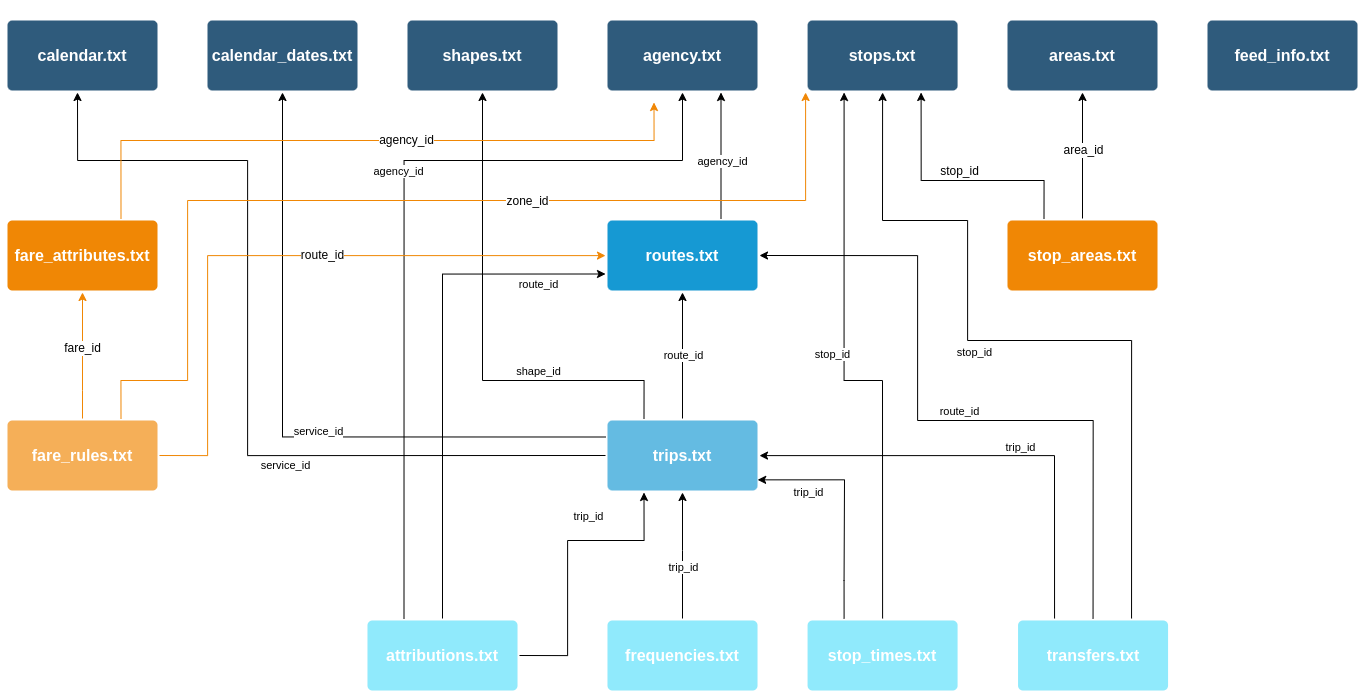
\includegraphics[width=1.0\textwidth]{GTFS Diagram}
    \caption{GTFS Dependencies}
    \label{fig:figure1}
\end{figure}

%\section{First Example}

\definecolor{gray}{rgb}{0.9,0.9,0.9}

\newpage
\subsection{GAIA Configuration}

\begin{justify}
There are two configuration files that are required by the application in order to work properly:
\begin{itemize}
\item \textbf{gaia.cfg}: with all global settings
\item \textbf{gtfs.cfg}: to be customised accordingly with data set and application needs.
\end{itemize}
\end{justify}

\subsubsection{Settings in gaia.cfg}

\begin{justify}
This configuration file contains all global settings such as directories to be used and settings for both logging and parser.
Let's see all of this sections in details starting from \textbf{\textit{global}}.
\end{justify}

\begin{small}
\begin{lstlisting}[backgroundcolor=\color{gray},frame=single]
global = {
  src_dir="gtfs_in/";
  dst_dir="gtfs_out/";
  feed_extension=".txt"
 
  logging = { ... };
  parser  = { ... };
}
\end{lstlisting}  
\end{small}

\begin{itemize}
\item \textbf{src\_dir}: specify \textit{source directory} where to find original \textbf{\textit{GTFS feeds}}.
\item \textbf{dst\_dir}: specify \textit{destination directory} used to write GTFS output feeds once all filters have been applied.
\item \textbf{feed\_extension}: file extension type for the \textbf{\textit{GTFS feeds}}.
\item \textbf{logging}: subsection containing general logging general settings.
\item \textbf{parser}: subsection containing general parser general settings.
\end{itemize}

\newpage
\subsubsection{global.logging}

In this subsection we can find all global settings for the logger.

\begin{small}
\begin{lstlisting}[backgroundcolor=\color{gray},frame=single]
  logging = {
    log_directory="log/";
    log_filename="_gaia.log";
    log_enable_console=true  
  };
\end{lstlisting} 
\end{small} 
\begin{itemize}
\item \textbf{log\_directory}: specify the directory where to write outputl logs. 
If specified directory does not exists it will be created.  
\item \textbf{log\_filename}: suffix appended to each log filename, more in general the\newline 
application will generate a new log file at each run and format used \newline
is \textbf{YYYYmmGGHHMMSS}, so final log filename will have the following\newline
form \textit{20221120104006\_gaia.log} where we have information about the\newline 
date \textbf{2022/11/20} and time \textbf{10:40:06} in which log have been generated.
\item \textbf{log\_enable\_console}: enable or disable log on standard output.
\end{itemize}

\newpage
\subsubsection{global.parser}

In this subsection are listed settings for the csv parser, such information will be used to initialize \href{https://github.com/fe-dagostino/libcsv}{\textit{\textbf{libcsv}}}.

\begin{small}
\begin{lstlisting}[backgroundcolor=\color{gray},frame=single]
  parser = {
    delimeter        = ",";
    quote            = "\"";
    eol              = "\n";
    comment          = "#";
    whitespaces      = "\a\b\t\v\f\r\n";
    skip_whitespaces = true;
    trim_all         = true;
    allow_comments   = false;
  };
};
\end{lstlisting}
\end{small}

\begin{itemize}
\item \textbf{delimeter}: characther used as \textit{field delimeter} when parsing \textit{csv} \textit{row}
\item \textbf{quote}: characther used as \textit{quote delimeter} when parsing the single \textit{field} in a \textit{row}
\item \textbf{eol}: End Of Line character used to identify when a \textit{row} has ended
\item \textbf{comment}: \textit{csv} standard do not make any mention for remarks inside the \textit{csv} itself, anyway the parser have this capability. 
\item \textbf{whitespaces}: define the list of whitespaces
\item \textbf{skip\_whitespaces} = \textit{enable}/\textit{disable} skip whitespaces. When true all whitespaces will be not anymore present in the \textit{output}.
\item \textbf{trim\_all}: \textit{enable}/\textit{disable} \textit{trim all}. When enabled all spaces at before and after a field will be removed unless the field is quoted.
\item \textbf{allow\_comments}: \textit{enable}/\textit{disable} comments inside the \textit{csv}.
\end{itemize}

\subsubsection{Settings in gtfs.cfg}

\begin{justify}
\end{justify}

\end{document}

